\chapter{Conclusion}
\label{chap:conclusion}

\graphicspath{{Chapter7/figures/}}

This chapter reviews the contributions that the thesis makes to support sensemaking through interactive visualizations of analytic provenance data. It also discusses opportunities for future research on analytic provenance for sensemaking.

\section{Review of Contributions}
The central problem addressed in this thesis is how to design interactive visualizations of analytic provenance data for supporting sensemaking. To address the problem, we proposed a process model, in which analytic provenance can be used to support the ongoing and iterative sensemaking process (\autoref{fig:intro-workflow}). The problem was then broken into four research questions based on the input and output of the provenance visualization component of the model: the type of data that would be visualized and the task it aimed to support, respectively. Each research question can be considered as an instance of the model, applied in different domain and context, showing the wide application of analytic provenance in supporting sensemaking. For each research question, we took a user-centered approach in designing the visualization to provide desired sensemaking support. The research process covered requirements analysis, visual encoding and interaction design, prototype implementation and user evaluation. 

Overall, the thesis contributes novel and validated interactive visualizations of analytic provenance data to support users in making sense of temporal and rational relationship. While users employ the sensemaking system to solve problems, their actions are automatically captured and their knowledge is externalized through manual annotation. Both these types of provenance data are visualized in ways that enable users to remind what has been done, to identify patterns and relationships in the data, to develop and refine understanding of the sensemaking problems, and to present and explain their findings effectively. \autoref{fig:con-contribution} summarizes the contributions by adding relevant highlights to \autoref{fig:intro-workflow}. Detailed contribution for each research question will be discussed next.

\begin{figure}[!htb]
	\centering
	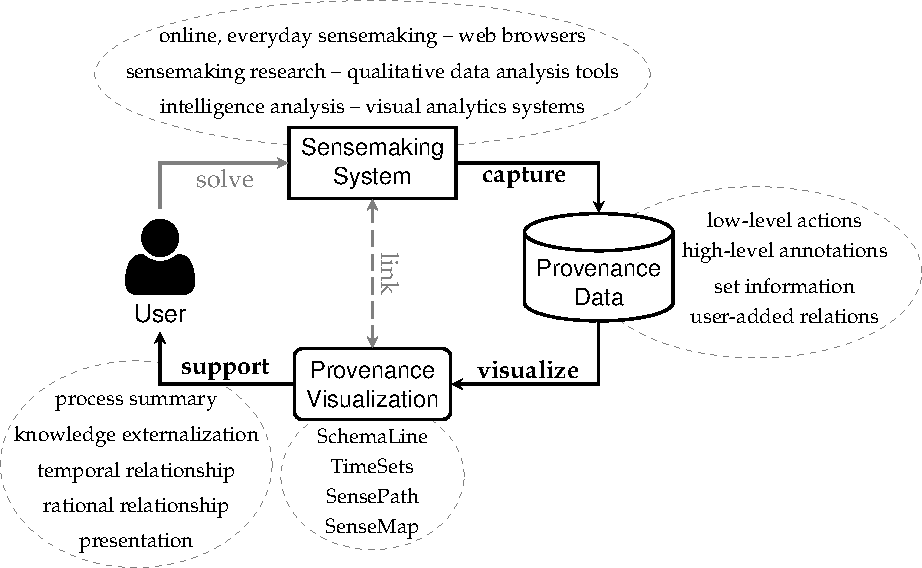
\includegraphics{contribution}
	\caption[Summary of thesis contributions]{Summary of thesis contributions. Relevant details (surrounded by dashed ellipses) are added into the original model in \autoref{fig:intro-workflow}. The thesis targets multiple domains showing a wide application of analytic provenance: intelligence analysis, sensemaking research and online everyday sensemaking. Different types of provenance data are visualized including automatically captured user actions, manual notes taken, set information, and spatial grouping and linking user-added relations. As a result, four interactive visualizations (SchemaLine, TimeSets, SensePath and SenseMap) are designed and evaluated to provide helpful sensemaking supports to the users including summarizing what has been done, allowing users to externalize their knowledge, gaining understanding of temporal and rational relationship in the sensemaking problems, and presenting the findings with support evidence.}
	\label{fig:con-contribution}
\end{figure}

\subsection{Exploring Temporal Relationship of Sensemaking}
\textbf{Research Question 1:} \emph{How to design interactive visualizations of timestamped provenance data that enables users to explore temporal relationship in sensemaking?}

We contributed a novel timeline visualization, SchemaLine, that enables users to explore temporal relationship in sensemaking through the annotations they made during the sensemaking processes. SchemaLine helps users examine the events recorded in those annotations in chronological order, identify interesting temporal patterns and construct narratives that account for those patterns. The SchemaLine visualization produces a compact but aesthetically pleasing layout. It also provides a set of fluid interactions supporting users in performing various sensemaking activities described in the Data--Frame model, such as connecting relevant data into an explanatory frame. Our user-centered evaluation showed that all participants found the SchemaLine visualization intuitive to use and it provided necessary support to them for solving their tasks. They extensively recorded their thoughts by note taking, constructed schemas to organize the notes and discovered insightful findings. The participants were also confident in presenting the stories they found and defending them through the use of SchemaLine. The limitation of SchemaLine includes its low scalability and the incapability of showing multiple-schemas annotations, which was addressed in the next research question.
	
\subsection{Exploring Complex Temporal Relationship of Sensemaking}
\textbf{Research Question 2}: \emph{How to design interactive visualizations that can reveal both temporal and categorical dimensions of provenance data and enable users to explore more complex temporal relationship in sensemaking?}

We contributed a novel timeline visualization, TimeSets, that enables users to explore complex temporal relationship of sensemaking by effectively representing both temporal and categorical provenance data. TimeSets visually groups events that shares the same set but still preserves their temporal order. It color codes the backgrounds of the entire sets to distinguish them and uses colored gradient backgrounds for the intersections among those sets. To handle a large number of events, TimeSets dynamically adjusts the level of detail for each event within a given display estate. A lab controlled experiment showed that TimeSets was significantly more accurate than a state-of-the-art method in performing temporal and categorical related tasks and was the preferred choice for aesthetics and readability. We also demonstrated the wide application of TimeSets in different domains: intelligence analysis and publication data exploration.

The major limitation of TimeSets is that it only shows intersections between vertically neighboring sets, which only accounts for a small portion of all possible combinations of intersections. The set ordering algorithm to maximize the number of shared events and interaction to reorder sets partially helped address this issue. Future research can focus on increasing the number of visible intersections, prioritizing more important intersections based on some metrics, and providing an overview of all intersections to suggest further exploration. Another limitation is the false impression that the set area indicates its number of events. However, besides the number of events, the set area also depends on the temporal distribution of its events and text length. To address this issue, we could deemphasize the visual appearance of the set area or design a new shape outline algorithm to ensure the set area truly reflects its size.

%\begin{itemize}
%	\item \emph{Set intersections}. The major limitation of TimeSets is that it only shows the intersections between vertically neighboring sets, which is a small portion of all possible combinations of intersections. The set ordering algorithm to maximize the number of shared events and interaction to reorder sets partially helped address this issue. Future research can focus on increasing the number of visible intersections, prioritizing more important intersections based on some metrics, and providing an overview of all intersections to suggest further exploration.
%	
%	\item \emph{Set area encoding}. The area of the representing set seems to be a very strong indicator of its size; i.e., number of events. However, it is not designed like that in TimeSets. Besides the number of events, the set area also depends on the temporal distribution of its events. To address this issue, we could deemphasize the visual appearance of the set area or design a new shape outline algorithm to ensure the set area truly reflect the its size.
%	
%	\item \emph{Multiple-set events}. In \autoref{chap:timesets}, we proposed four different visual representations of multiple-set events (\autoref{sub:ts-eventmembership}). However, it is not clear which representation is the most effective and for which tasks. Therefore, a formal evaluation is necessary to examine this aspect.
%	
%	\item \emph{Aggregated events}. In the current TimeSets, there is no extra visual cue to help viewers quickly see the difference between the sizes of the aggregated events: they have to read the label. We proposed four different visual representations to display aggregations (\autoref{sub:ts-scalability}). However, similar to the previous point, a formal evaluation needs to be conducted to further investigate this design.
%\end{itemize}


\subsection{Exploring Rational Relationship of Sensemaking}
\textbf{Research Question 3}: \emph{How to design interactive visualizations of timestamped provenance data that enables analysts to explore rational relationship in sensemaking performed by other users?}

We contributed a novel visualization tool, SensePath, that enables analysts to explore the rational relationship in the sensemaking processes performed by other people. To understand such relationship, analysts often carry out a time-consuming qualitative study and analysis including data collection, transcription, coding and theory abstraction. SensePath offers an alternative and possibly faster approach in performing transcription and coding. It detects and captures user's sensemaking actions automatically, thus make it possible to generate an automatic transcript. SensePath also provides multi-linked visualizations of the captured actions, allowing the analysts to gain deep understanding of the rational relationship between these actions, thus facilitate the coding process. More specifically, a timeline view allows analysts to quickly gain an overview of the sensemaking process and identify recurring patterns. It also links with a screen capture video to support a close examination of additional context when necessary. Finally, to enable analysts to continue working on later stages of analysis using their normal workflow, SensePath exports its coded transcript in a common format that can be used by other popular qualitative data analysis software packages such as InqScribe. An evaluation with one experienced qualitative researcher showed the usefulness of SensePath in supporting the analysis by the researcher. Another evaluation with two HCI researchers suggested the potential of improvement in completion time for SensePath in the transcription and coding phases.

SensePath currently lacks a practical feature set of coding analysis. It facilitates coding through exploration of rational relationship of captured actions; however, it only supports simple code assignment and editing. The analyst can select an action and assign a new code or select from used ones. In practice, analysts could require more convenient and sophisticated features such as the following ones.
	\begin{itemize}
		\item Assign a code to a part of an action or a range of actions.
		\item Assign multiple codes to an action.
		\item Support hierarchical codes.
		\item Show the codes in the timeline view more effectively.
	\end{itemize}
	

\subsection{Exploring Complex Rational Relationship of Sensemaking}
\textbf{Research Question 4}: \emph{How to design interactive visualizations of timestamped provenance data that can incorporate user-added relations and enable users to explore more complex rational relationship in sensemaking?}

We contributed a novel visual sensemaking tool, SenseMap, that enables users to explore complex rational relationship of sensemaking. It automatically captures sensemaking actions and linking relationships between these actions before visualizing both of them in a branching history tree. The temporal attribute of actions is also partially reflected in the visualization. This history tree allows users to examine the rational relationship between the actions they performed and potentially helps them remind of what have been done earlier. SenseMap offers users to assign additional meaning to the automatically collected data by spatially grouping actions or adding rational links between them, in order to help explain complex relationship. Finally, SenseMap allows users to communicate their analysis results at different levels of granularity including a big picture of user-organized findings, a more detailed analysis process and raw provenance data captured. We conducted a user-centered evaluation in a naturalistic setting to explore how SenseMap would be used. The results showed that all participants found the visual representation and interaction of the tool intuitive to use. Participants who were engaged positively with the tool produced successful sensemaking outcomes. It helped them organize information sources, quickly find and navigate to the sources they wanted, and effectively communicate their findings.

The major limitation of SensePath is its low user engagement. Two participants in the evaluation did not engage with the tool and led to a poor sensemaking performance. One of the reasons was their computer screen sizes were not large enough to show all three views at the same time, and they were unable to switch between the views comfortably to keep track of the history map construction. A possible improvement is to design a more space-efficient history map so that it can display side by side with the browser view. Another option is to allow users to focus on the browser view, but provide sufficient feedback to help them understand the map development. Also, a visual summary of changes in the map could also help users catch up more quickly.

The evaluation showed that SenseMap provided useful sensemaking support for users in a 2-hour-long session. However, in the real world, a sensemaking task can be split into small chunks and spanned multiple days or even weeks. A larger scale and longer term study is necessary to gain better understanding of SenseMap's use. Because SenseMap is implemented as a Chrome extension that available to all Chrome users, this gives us a good opportunity to conduct such a study.

\section{Future Direction}
We suggest the following future research that can have a high impact on supporting sensemaking through analytic provenance.

\paragraph{Automatic inference of sub-tasks from actions}
User actions such as ``search'' and ``filter'' can be captured automatically but they provide little semantics. A large number of actions poses a challenge in visualizing and summarizing the sensemaking processes, preventing users from quickly understanding what has been done. Therefore, it is important to generate a high-level summary of low-level actions automatically. This problem is a huge challenge and might be impossible to design a generic and automatic algorithm to produce such an inference. Focusing on a particular sensemaking task in a specific domain could make the inference more feasible thus could be a good starting point.

\paragraph{Specific sensemaking tasks support}
The thesis supports sensemaking in multiple domains; however, it does not target a specific sensemaking task in depth. For example, SenseMap is designed to support people in making sense of their everyday problems such as selecting a suitable smartwatch. A specific task in solving such a problem could be comparison of different models. Supporting specific tasks aim to produce actionable information to the users, enabling them to make more informed decisions.

\paragraph{General visualization challenges}
Addressing challenges in visualizing analytic provenance will also benefit a large community. Currently, the History Map in SenseMap uses a tree layout with node location implying temporal order between a subset of nodes such as nodes in a path growing from left to right. How to embed temporal information in all nodes effectively? This is the general problem of visualizing time-oriented networks. Similarly, the problem of visualizing temporal, multiple-set relations in TimeSets could benefit many different domains and should attract more research effort.

\section{Closing Remarks}
The data around the world has been produced more rapidly than ever before. It could provide us a good opportunity to collect more relevant information for solving our problems, but also challenge us in analyzing a large dataset and synthesizing a large number of individual findings. Analytic provenance captures the actions and accompanied reasoning in the sensemaking process. The captured data is then visualized to help the user recall the process, understand the temporal and rational relationship in the solving problem more deeply, and potentially suggest the next step in sensemaking. A deep understanding about the past could lighten the future. This thesis contributes novel visualizations to support people making sense of their tasks more effectively and opens more research in this direction.